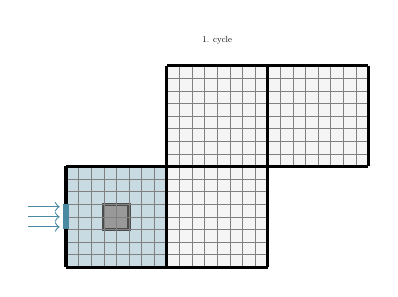
\begin{tikzpicture}
[
scale=0.32,
every node/.style ={scale=0.32},
Background/.style={rectangle,draw=black!04,fill=black!04, thin, minimum size = 4 cm},
BackgroundInflow/.style={rectangle,draw=black!04,fill={rgb,255:red,73;green,137;blue,162},opacity=0.3, thin, minimum size = 4 cm},
Obstruction/.style={rectangle,draw=black!70,fill=black!40, very thick, minimum size=1cm},
Finegrid/.style={step=0.5cm,gray,very thin},
Thickline/.style={-,draw=black!100,fill=black!02, very thick},
Thinline/.style={draw=black!100,fill=black!02, very thin},
Inflow/.style={-,draw={rgb,255:red,73;green,137;blue,162},line width=0.8mm},
Inarrow/.style={->,draw={rgb,255:red,73;green,137;blue,162},thin},
Outflow/.style={-,draw=blue!60,,line width=0.8mm},
Ball/.style={circle, draw=black!40, fill=red!20, thin, minimum size=3.5mm},
Circle/.style={circle,draw=black!40,fill=black!06,thin,minimum size=35.5mm},
Rectangle/.style={rectangle,draw=black!10,fill=white,inner xsep=0pt, inner ysep=0pt,},
Box/.style= {very thin, rectangle, inner xsep=10pt, inner ysep=10pt,},
ComArrow/.style={<->,semithick,draw=red!70},
]

\node[BackgroundInflow] at (2,2) {};
\node[Background] at (6,2) {};
\node[Background] at (6,6) {};
\node[Background] at (10,6) {};

\node[Obstruction] at (2,2) {};

\draw[Finegrid] (0,0) grid (8,4);
\draw[Finegrid] (4,4) grid (12,8);

\draw[Thickline] (0,0)--(8,0);
\draw[Thickline] (4,8)--(12,8);
\draw[Thickline] (0,4)--(4,4);
\draw[Thickline] (8,4)--(12,4);

\draw[Thickline] (0,0)--(0,4);
\draw[Thickline] (4,8)--(12,8);
\draw[Thickline] (4,4)--(4,8);
\draw[Thickline] (8,0)--(8,4);
\draw[Thickline] (12,4)--(12,8);

\draw[Thickline] (4,0)--(4,4);
\draw[Thickline] (4,4)--(8,4);
\draw[Thickline] (8,4)--(8,8);

\draw[Inflow]   (0,1.5)--(0,2.5);
\draw[Inarrow]  (-1.5,1.6)--(-0.25,1.6);
\draw[Inarrow]  (-1.5,2.0)--(-0.25,2.0);
\draw[Inarrow]  (-1.5,2.4)--(-0.25,2.4);
%\draw[Outflow]  (12,4)--(12,8);

%\draw[ComArrow](3.0,2)--(5.0,2);

\node [Box] (Box) at (6.0,9.0){{\HUGE 1. cycle}};

\end{tikzpicture}
